%%%%%%%%%%%%%%%%%%%%%%%%%%%%%%%%%%%%%%%%%%%%%%%%%%%%%%%%%%%%%%%%%%%
%                                                                 %
%                            CHAPTER FOUR                          %
%                                                                 %
%%%%%%%%%%%%%%%%%%%%%%%%%%%%%%%%%%%%%%%%%%%%%%%%%%%%%%%%%%%%%%%%%%%

\chapter{VERIFICATION} \label{sec:verification}

% \section{Viewpoint \& Quality Verification}

\begin{figure}[t]%
%\begin{figure}[!htb]%
    \centering
    \subfloat {{ $\vcenter{\hbox{ 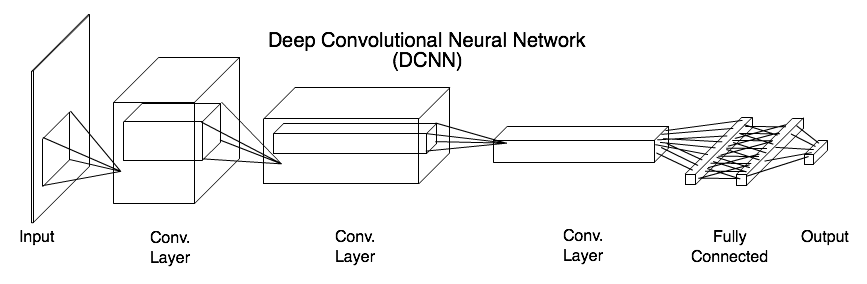
\includegraphics[width=0.90\textwidth]{resources/dcnn.png} }}$ }}%
        \caption[The Structure of a Deep Convolutional Neural Network (DCNN)]{\textbf{The Structure of a Deep Convolutional Neural Network (DCNN).}  A DCNN architecture is a neural network utilizing multiple convolutional layers to reduce the image into a small convolutional feature vector.  The convolutional feature vector is then classified using fully-connected layers, which terminates with a Softmax activation.  DCNN-based techniques are the current state-of-the-art for whole image classification, alongside a multitude of computer vision applications.}
        \label{fig:dcnn}
\end{figure}

To verify the viewpoint and quality annotations produced during the analysis, we designed a Deep Convolutional Neural Network (DCNN) to classify image patches and identify inconsistencies.  A neural network is a hierarchical collection of neural layers, which are comprised of neural units.  Each neural unit has the following structure: an input, learned weights, a learned bias, an activation function, and an output.  The input to a neural unit is used, along with its matrix (or vector) of learned weights, to produce a single number result through a matrix dot product operation.  In a traditional (fully-connected) neural unit, all input values are applied to a single weight matrix, which means that there is a one-to-one correspondence between every value in the learned weight matrix and every input value.  The dot product result is added to the learned bias term and then passed as input to the specified activation function for that neural unit.  The output of the activation function is the output of the neural unit.  This structure is formalized in Equation \ref{eq:fully-connected}.  The activation function should be non-linear; a non-linear activation function allows the network to learn complex approximations of high-dimensional data.  The non-linearity also allows the network to  become deeper and therefore capture more complex representations in the input data \cite{glorot_deep_2011, hecht-nielsen_theory_1989, krizhevsky_imagenet_2012}.

A neural layer is a collection of multiple neural units, where each unit is independently applied to the input for that layer.  A neural network is a hierarchical collection of neural layers, where the output of a previous layer is given to a subsequent layer as input -- forming a chain of neural layers.  The network takes as input an image to the first layer and produces a singular value as output to the last layer, using the Softmax function as its activation.  All intermediate layers that are not the input layer nor the output layer are called \textit{hidden layers} \cite{funahashi_approximate_1989}.

A DCNN is a special type of neural network where the structure is \textit{deep} (i.e.\ having more than one hidden layer) and \textit{convolutional} (i.e.\ utilizing \textit{convolutional layers} in the network's structure).  A convolutional layer differs from a fully-connected neural layer in that only a small subsection of the input is applied to the learned weight matrix.  As a result, the learned weight matrix is much smaller than the input and does not have a one-to-one correspondence.  However,  the weight matrix is convolved across the entire input along its spatial dimensions, as shown in Equation \ref{eq:convolution}.  Instead of producing a series of singular values like in a fully-connected neural layer, a convolutional layer produces a \textit{spatial} output; the spatial output is a resampling of the input using the convolutional layer's learned convolutional filters (weights).  Therefore, having multiple convolutional filters within a convolutional layer creates a series of image channels as output.

Let $H_c^\ell$ be the \textit{spatial} output for the convolutional neural unit of the $c$\th\ channel of layer $\ell$.  Furthermore, let $C^{\ell}$\ be the total number of feature channels in the $\ell$\th\ layer.  Let $W_{k,c} \in \mathbb{R}^{n \times m}$ be the learned weight matrix between the $k$\th\ channel of layer $\ell - 1$\ and $c$\th\ channel of layer $\ell$.  Let $b_{c}^\ell$ be the bias term for the entire channel $c$ of layer $\ell$.\footnote{This bias term is ``tied'' across all input channels, meaning channels share the same bias term for the entire convolutional filter.  Untied bias terms would be learned for each incoming filter and the bias would take the form $b_{k,c}^\ell$\ and should be incorporated into the summation.}  The values $n$ and $m$ define the size of the convolutional filter for that layer, where normally $n = m$.  The convolutional operation is represented using the asterisk operator $\conv$ with spatial stride $x$ and $y$, where also normally $x = y$.  The nonlinear activation function of the convolutional $\ell$\ layer, $f^\ell$,\ is used to compute the spatial activation output, given by the following equation:

\begin{equation}
    \label{eq:convolution}
    H_c^\ell = f^\ell \left(\sum_{k=1}^{C^{\ell - 1}} [ H_k^{\ell-1} \conv W_{k,c}^\ell ] + b_{c}^\ell \right)
\end{equation}

To see the computational differences between a convolutional layer and a fully connected layer, let's next consider the activation of a single neural unit in a fully-connected neural layer.  Let $h_j^\ell$\ be the output activation \textit{value} of the $j$\th\ neural unit in layer $\ell$.  Let $w_{i,j}^\ell$\ be the learned weight between $h_i^{\ell - 1}$\ and $h_j^\ell$.  Let $b_j^\ell$ be the bias term for the $j$\th\ neural unit in layer $\ell$.  Lastly, let $L^{\ell}$ be the number of neural units in the neural layer $\ell$\ and $f^\ell$\ be the nonlinear activation function for layer $\ell$.

\begin{equation}
    \label{eq:fully-connected}
    h_j^\ell = f^\ell \left(\sum_{i=1}^{L^{\ell - 1}} [ h_i^{\ell - 1} w_{i,j}^\ell ] + b_j^\ell\right)
\end{equation}

As we can see, the number of weights to learn for a fully connected layer is $\mathcal{O}(L_{\ell - 1} \cdot L_{\ell})$, whereas the number of weights to learn for a convolutional layer is $\mathcal{O} (C_{\ell - 1} \cdot C_{\ell} \cdot n \cdot m)$.  The number of fully-connected weights grows geometrically as more units are added to the network for representational power.  Conversely, the convolutional layers grow in only the size of the filters and the number of channels.  An important distinction is that the number of weights learned by the network for convolutional layers is fixed, independent of the size of the input, which allows a convolutional network to be trained faster and have overall far fewer learned parameters compared to a fully-connected network.

Mixed in with the convolutional layers, the DCNN utilizes max-pooling layers, which summarizes a pooling area by simply taking its maximum value.  Max pooling layers, by definition, do not have any learned weights or a bias value.   Max-pooling layers are used to reduce the spatial dimensions of the input, which reduces the computational cost of the DCNN and provides a degree of translation invariance \cite{lee_convolutional_2009, riesenhuber_models_2000}.  The convolutional and pooling layers also act as a form of regularization as it decreases the total number of parameters in the network, reducing the possibility of overfitting the training data.  A DCNN is generally comprised of a series of mixed convolutional layers and max-pooling layers followed by a series of fully-connected neural layers.  See Figure \ref{fig:dcnn} for a diagram of an abstracted DCNN.

To perform automatic viewpoint and quality labeling, we trained two Deep Convolutional Neural Networks: one network to label viewpoints of zebras and another network to determine the qualities of the zebra images.  These two networks were trained using CUDA \cite{nickolls_scalable_2008}, Theano \cite{bastien_theano:_2012, bergstra_theano:_2010}, and Lasagne \cite{dieleman_lasagne:_2015} on an NVIDIA GTX 660 GPU.  The resulting trained models were integrated into the IBEIS infrastructure in order to suggest species, viewpoint, and quality information for future collected data.

%\subsection{DCNN Architecture}
\section{DCNN Architecture}
The architecture of our DCNN followed the design paradigms established in most recent neural network literature.  The network used mini-batching \cite{hinton_fast_2006} to average training examples given to the network, stochastic gradient decent (SGD) \cite{gardner_learning_1984, tsitsiklis_distributed_1986} to optimize the network parameters, Nesterov's momentum \cite{nesterov_method_1983} (momentum with exponential averaging and a peak-ahead value that attempts to smooth the convergence of SGD) with a value of 0.9, Rectified Linear Units (ReLU) \cite{dahl_improving_2013, krizhevsky_imagenet_2012, nair_rectified_2010} as the activation functions, dropout \cite{hinton_improving_2012} in all layers (including convolutional layers), MAXOUT \cite{goodfellow_maxout_2013} (feature pooling) in the fully-connected layers, orthogonal weight initialization \cite{saxe_exact_2013}, and a cross-entropy error gradient.  The network used 3x3 convolutional filters after the first two layers (densely convolved across with a stride of 1x1) and used non-overlapping max-pooling of size 2x2 with a stride of 2x2.  During training, a patience threshold was used to govern the learning rate schedule; if the validation error stopped decreasing, we waited the patience number of epochs before decreasing the learning rate \cite{fahlman_cascade-correlation_1990}.  For all of our training, we reduced the learning rate by half after the validation stopped improving.  The architecture used for both the viewpoint and quality neural networks is described in Table \ref{tab:architecture}.

\begin{table}[!ht]
    \centering
        \caption[Deep Convolutional Neural Network (DCNN) Architecture by Layer]{\textbf{Deep Convolutional Neural Network (DCNN) Architecture by Layer.}  The DCNN architecture was used for both the viewpoint and quality labeling networks.  The initialization for layers 1 and 2 used the pre-trained CaffeNet model, convolutional layers 1 and 2; layers 3 and deeper used orthogonal (ortho.) weight initialization.  The network was allowed to fine-tune the initialized CaffeNet model.  Dropout was used in all layers except for the transition between convolutional and fully-connected as we did not want to alter the convolutional feature vector seen by the dense layers.  A Maxout feature pooling layer was added in the fully-connected layers to pool between the strongest feature out of 512 channels with a neighborhood of 2.  The three output sizes correspond to the 8-class zebra viewpoint, 5-class zebra quality, and the full 40-class (8 viewpoints for 5 species) species and viewpoint classification networks.}
        \resizebox{\linewidth}{!}
    {
        \begin{tabular}{l|ccccc|cc|c}
                \hline
                & & & & & & & & \head{Output} \\
                \head{Layer} & \head{1} & \head{2} & \head{3} & \head{4} & \head{5} & \head{6} & \head{7} & \head{8} \\
                \hline
                Stage & conv. & conv. + max & conv. + max & conv. + max & conv. + max & full & full & full \\
                \# channels & 32 & 32 & 64 & 128 & 128 & 512 & 512 & 8/5/40 \\
                Filter size & 11x11 & 5x5 & 3x3 & 3x3 & 3x3 & - & - & - \\
                Conv. stride & 1x1 & 1x1 & 1x1 & 1x1 & 1x1 & - & - & - \\
                Pooling size & - & 2x2 & 2x2 & 2x2 & 2x2 & - & - & - \\
                Pooling stride & - & 2x2 & 2x2 & 2x2 & 2x2 & - & - & - \\
                Zero-Padding size & - & - & 1x1x1x1 & 1x1x1x1 & - & - & - & - \\
                Dropout & 0.10 & 0.10 & 0.30 & 0.30 & - & 0.50 & 0.50 & - \\
                Maxout (feat. pool) & - & - & - & - & - & 2 & 2 & - \\
                Initializer & CaffeNet (0) & CaffeNet (1) & ortho. & ortho. & ortho. & ortho. & ortho. & ortho. \\
                \hline
                Spatial input size & 96x96 & 86x86 & 41x41 & 20x20 & 9x9 & 3x3 & 1x1 & 1x1 \\
        \end{tabular}
    }
        \label{tab:architecture}
\end{table}

The network was trained by taking every annotation from the analysis phase and cropping out the individual animal from the rest of the image to create a patch.  The resulting cropped patch was then resized to 96x96 pixels (ignoring aspect ratio) and then saved to disk.  The images were then loaded into a 4D Numpy \cite{van_der_walt_numpy_2011} structure, which held all of the square image patches.  A corresponding ground-truth 1D parallel Numpy structure was also generated, which held an encoding of the correct species and viewpoint for each image patch.  The total dataset was split into a training and validation set, with the validation set containing 20\% of the training examples.  The validation data was used to control overfitting by utilizing early-stopping and provided an unbiased accuracy metric for the network.  The images were given to the network as input in mini-batches of size 128, was trained with an initial learning rate of 0.1, and utilized an L2 regularization of 0.0001 on the error gradient.  The network optimized the parameters (weight matrices and bias terms) of the network using SGD and back-propagation \cite{rumelhart_learning_1986} to learn the representation of the pixel data and classify the image patches into 8 categories, one for each of the 8 viewpoints: \textit{left}, \textit{back-left}, \textit{back}, \textit{back-right}, \textit{right}, \textit{front-right}, \textit{front}, and \textit{front-left}.  The correct orientation of the animal was encoded as a \textit{one-hot} vector (i.e.\ a vector where each classification category occupies one index of the vector and the correct category is set to 1 and all other categories are set to 0) and compared to the one-hot vector ground-truth during network training.   The cross-entropy error gradient was calculated recursively starting from the last, output layer working towards the input layer and averaged across all of the training examples in the mini-batch.  Mini-batch averaging not only tempers the randomness of the error gradient for each example, but also makes computing the gradient computationally efficient on GPU hardware.

\begin{figure}[t]%
%\begin{figure}[!htb]%
    \centering
    \subfloat {{ $\vcenter{\hbox{ 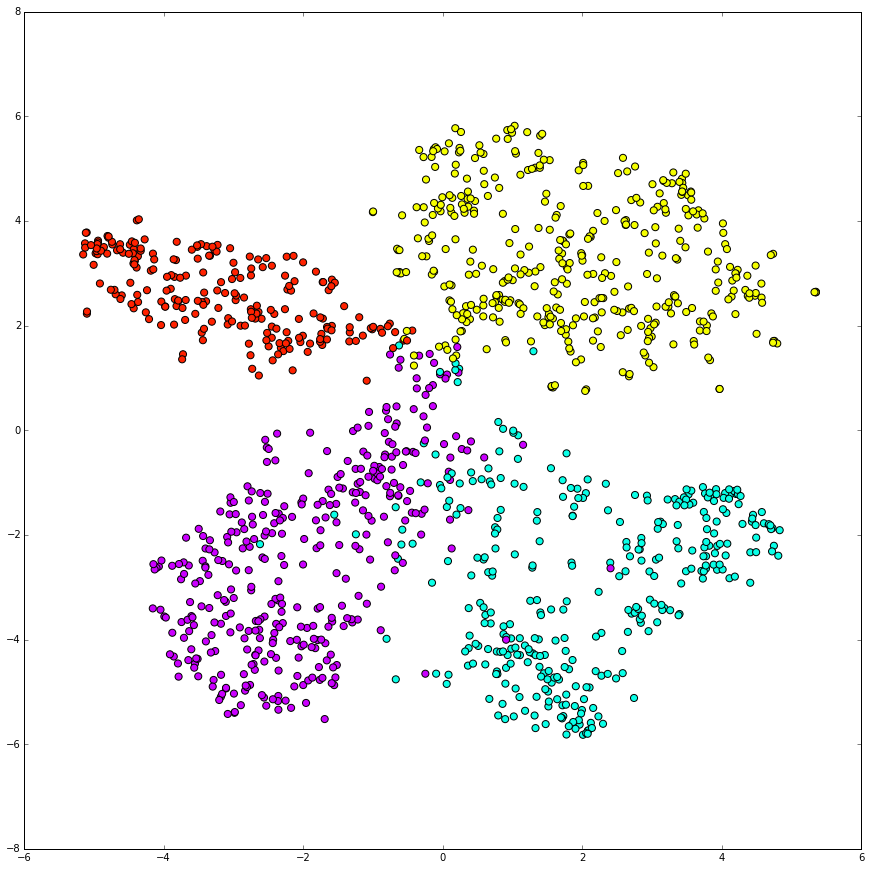
\includegraphics[width=0.45\textwidth]{resources/tsne-species.png} }}$ }}%
    \subfloat {{ $\vcenter{\hbox{ 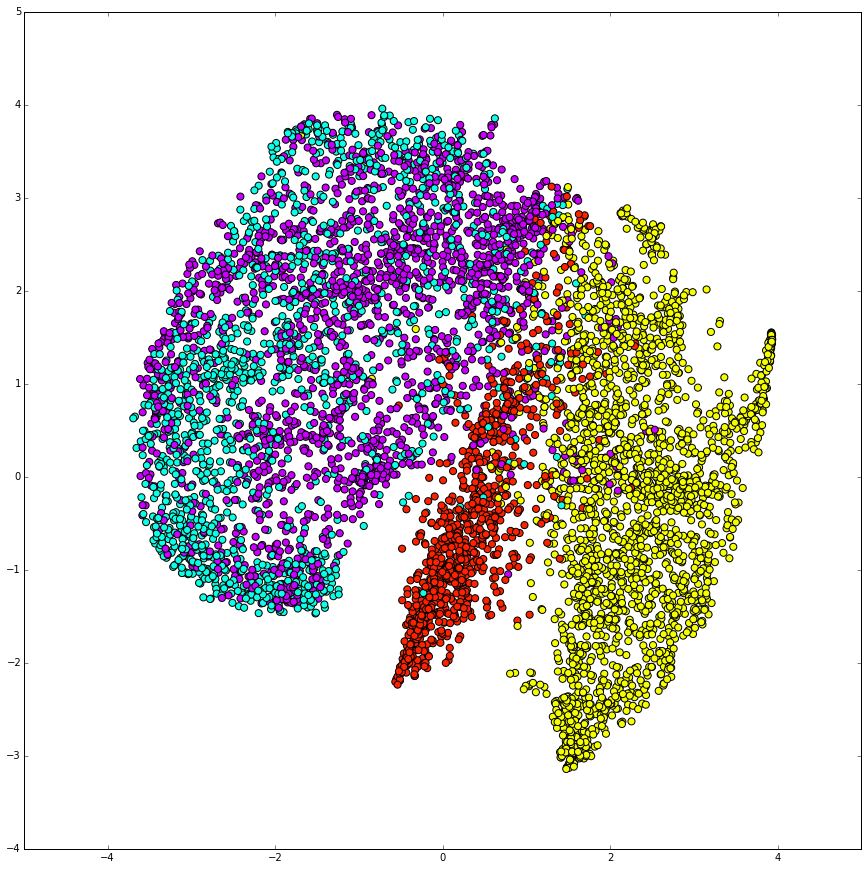
\includegraphics[width=0.45\textwidth]{resources/tsne-without-negatives.png} }}$ }}%
        \caption[t-SNE on CaffeNet Convolutional Feature Vectors]{\textbf{t-SNE on CaffeNet Convolutional Feature Vectors.}  The convolutional feature vectors were extracted as the output of the last convolutional layer from the CaffeNet model.  The feature vectors were extracted on images of African elephant (red), reticulated giraffe (yellow), Grevy's zebra (blue) and plains zebra (purple).  Feature vectors were extracted on 227x227 pixel resized (ignoring aspect ratio) square images of the sightings (left) and 227x227 pixel square (no resizing) patches taken as random croppings out of the sightings (right).  It should be noted that the stock CaffeNet model has little trouble producing separable features for full images of animals, but has trouble separating cropped patches of Grevy's and plains zebra considering their similar visual appearance.}
        \label{fig:tsne}
\end{figure}

The network was initialized using pre-trained layers from the CaffeNet model, which was trained on the ILSVRC dataset \cite{russakovsky_imagenet_2015} and released using Berkley's Caffe \cite{jia_caffe:_2014} neural network framework.  Our implementation used the Theano and Lasagne neural network frameworks, but was compatible with the learned models released by Caffe through a Caffe-to-Lasagne converter\footnote{github.com/kitofans/caffe-theano-conversion [Accessed: Nov. 1, 2015]}.  Using Lasagne, the first two layers of our network were initialized using the first two layers of the CaffeNet model.  Our network was allowed to fine-tune these initialized layer parameters; fine-tuning transferred layer parameters has shown to produce better overall accuracy compared to keeping the weights fixed during training \cite{yosinski_how_2014}.  All other layers (layer 2 and deeper) were initialized randomly using orthogonal weight initialization.  The transferred learning \cite{oquab_learning_2014} allowed the network to not only quickly converge, but the general convolutional filters learned from the ImageNet dataset improved the neural network's ability to classify the image patches correctly.

The CaffeNet model is Berkley's implementation of the network trained by Krizhevsky et al., named AlexNet \cite{krizhevsky_imagenet_2012}, on the ImageNet ILSVRC data.  The model was trained on the 1,000 classes defined by the ImageNet ILSVRC, which offers 1.2 million images to train the neural network.  The expansive amount of training data and classes can be used to train a model with general features, features general enough to also be applied against classes that were not explicitly given during training.  For example, the ILSVRC 2012 training data contains classes for plains zebra and African elephant, but does not have specific training examples for any species of giraffe or Grevy's zebra.   However, as shown in Figure \ref{fig:tsne}, the trained CaffeNet model and learned convolutional features can still be effective in classifying images containing giraffes and Grevy's zebras.  Convolutional feature vectors can be produced by the CaffeNet as the output of the last convolutional layer, just before the fully-connected layers.  Using the CaffeNet model, we extracted convolutional features on images of African elephant (\textit{Loxodonta}), reticulated giraffe (\textit{Giraffa camelopardalis reticulata}), Grevy's zebra (\textit{Equus grevyi}) and plains zebra (\textit{Equus quagga}).  The resulting feature vectors are visualized using t-SNE (t-Distributed Stochastic Neighbor Embedding) \cite{van_der_maaten_visualizing_2008} in Figure \ref{fig:tsne} (left); t-SNE is a machine learning algorithm for performing dimensionality reduction that provides a method to visualize the high-dimensional feature vectors in two dimensions better than performing PCA \cite{jolliffe_principal_2002}.  As we can see, the convolutional layers produced feature vectors that offer a high degree of separability between the different species.

\begin{figure}[t]%
%\begin{figure}[!htb]%
    \centering
    \subfloat {{ $\vcenter{\hbox{ 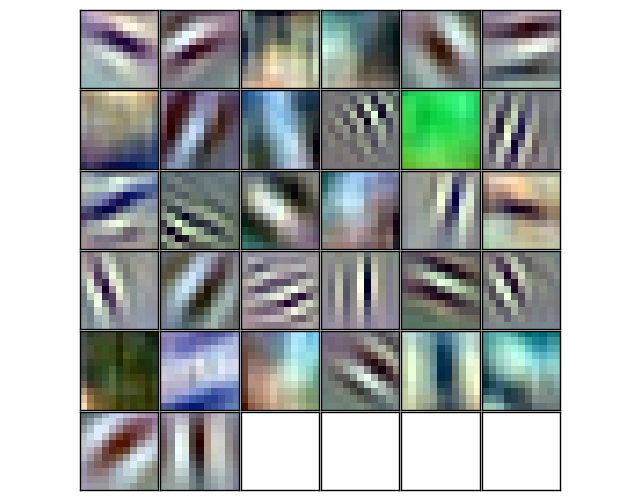
\includegraphics[width=0.45\textwidth]{resources/features_conv0_epoch_0_color.png} }}$ }}%
    \subfloat {{ $\vcenter{\hbox{ 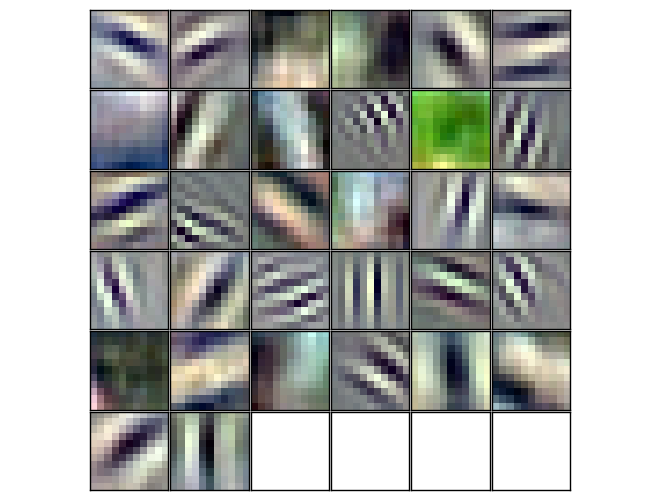
\includegraphics[width=0.45\textwidth]{resources/features_conv0_epoch_199_color.png} }}$ }}%
        \caption[First Convolutional Layer Features from CaffeNet]{\textbf{First Convolutional Layer Features from CaffeNet.}  The features from the first convolutional layer of the CaffeNet model at the start of training (left) have more color variations compared to the fine-tuned features at the end of training (right).}
        \label{fig:features}
\end{figure}

To produce the feature vector visualizations, the image patches were resized (ignoring aspect ratio) to 227x227.  As we can see, when given full images of the animals the network does not have any problem separating between sub-species of zebras, African elephant, and the unrepresented category of giraffe.  Furthermore, the network also provides sufficient separability between the two sub-species of zebra, which are the most similar in visual appearance.  The ease of the stock CaffeNet model in separating between previously unseen categories, even the nuanced visual differences between different sub-species, gives hope that a network could be trained to distinguish between different viewpoints of the same species.  In Figure \ref{fig:tsne} (right), feature vectors were also visualized for 227x227 pixel square patches taken as random crops out of the annotation images.  Notably, the network does have a hard time classifying between subsampled patches of plains zebra (purple) and grevy's zebra (blue), which are visually similar and hard to distinguish without having a complete context to differentiate the species.  This suggests that local information is insufficient to classify between sub-species of zebra.

\section{Viewpoint and Quality Labeling}
%\subsection{Viewpoint \& Quality Labeling}

\begin{figure}[t]%
%\begin{figure}[!htb]%
    \centering
    \subfloat {{ $\vcenter{\hbox{ 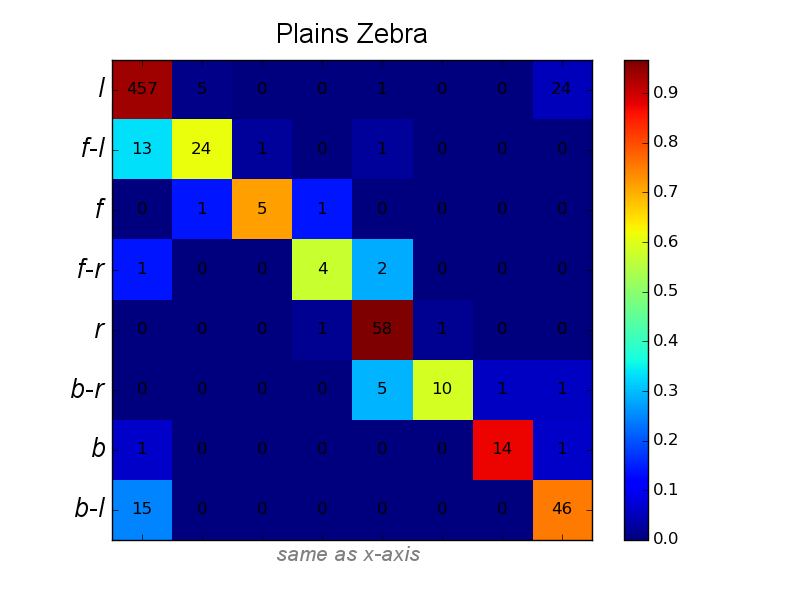
\includegraphics[width=0.45\textwidth]{resources/confusion-viewpoint-cleaned.png} }}$ }}%
    \subfloat {{ $\vcenter{\hbox{ 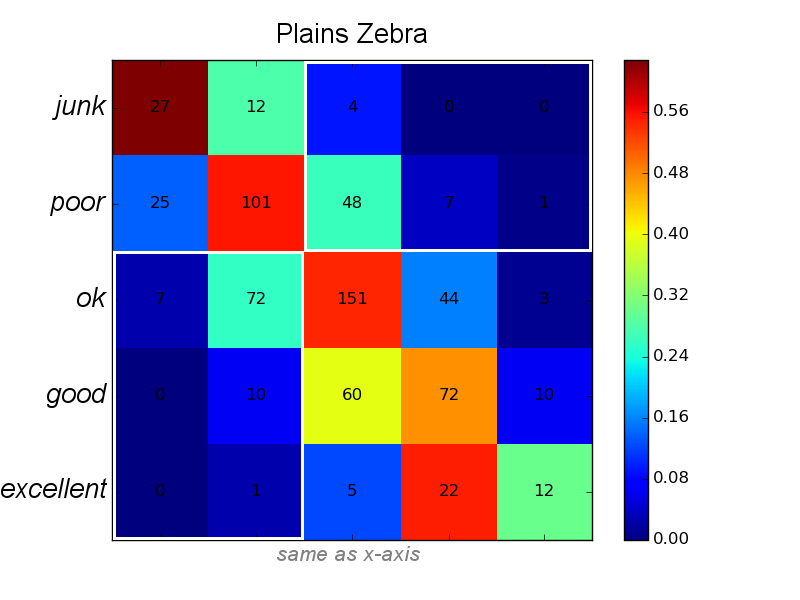
\includegraphics[width=0.45\textwidth]{resources/confusion-quality-cleaned.png} }}$ }}%
        \caption[Confusion Matrices for Viewpoint and Quality DCNN]{\textbf{Confusion Matrices for Viewpoint and Quality DCNN.}  The confusion matrices for both the viewpoint (left) and the quality (right) DCNN architectures at the end of training on plains zebras.  The network has little trouble distinguishing between the different viewpoints of zebra using the fine-tuned CaffeNet model.  Conversely, the network has quite a bit of trouble classifying the fuzzy quality metric, which is largely subjective between reviewers.  Note that the scales are different between the two confusion matrices.}
        \label{fig:confusion}
\end{figure}

Verifying the annotated viewpoints was required because the identification pipeline relied heavily on viewpoint information to accurately identify sighted animals and filter results.  For example, a viewpoint of a right hand-side was filtered during identification such that left hand-side matches were intentionally disregarded.  A viewpoint labeling DCNN was trained using a total of 8,660 annotations of plains zebras.  These annotations were binned into the 8 cardinal and sub-cardinal viewpoints: \textit{left} (6085), \textit{front-left} (755), \textit{front} (85), \textit{front-right} (88), \textit{right} (751), \textit{back-right} (212), \textit{back} (201), and \textit{back-left} (755).  The viewpoints of zebra collected during the GZGC were obviously heavily skewed towards the left viewpoint due to the collection protocol.  However, during training the data was augmented by performing horizontal flipping of the image pixels to artificially generate new training examples between left and right.  This data augmentation exploits the approximate left-right symmetry of zebras (and giraffes).  Conversely, identification cannot exploit this approximation since it relies too heavily on specific visual information, which is not left-right symmetric.  This augmentation obviously helped to resolve some of the class imbalance, but unfortunately the front and back viewpoints were painfully under-sampled.  However, the network still obtained compelling performance in classifying all seen viewpoints of zebras.

The initialized CaffeNet features shown in Figure \ref{fig:features} (left) were fine-tuned by the DCNN in order to allow the network to learn a better representation for our dataset.  By the end of training the viewpoint network, the convolutional filters had changed to accommodate less color variation and focus on more black-to-white comparisons.  As seen in Figure \ref{fig:features} (right), The desaturation of the filters is hypothesized to be due to over half of the image patches given to the network are of plains and Grevy's zebras, which obviously do not contain much color variation.  It is noteworthy that the green filter changed to a deeper green, which closer matches the background vegetation color from the negative background patches given to the network during training.  It should also be noted that the convolutional features are roughly identical to where they were initialized, meaning that either the network could not escape the local minimum during training or that the network found these filters to be satisfactory in classifying the image patches.  However, the general blurriness of the convolutional filters suggest that these 11x11 initial filters are too large, which supports the claims and performance increases seen in more recent networks \cite{bengio_advances_2013, sermanet_overfeat:_2013, simonyan_very_2014, springenberg_striving_2014, szegedy_going_2014} that smaller convolutional filters are better for convolutional-based classification.

As seen in the confusion matrix in Figure \ref{fig:confusion} (left), the network did a decent job in distinguishing between the different viewpoints of zebra, resulting in an overall validation accuracy of 89.05\%.  The viewpoint network was applied to the training data and successfully identified mis-annotated species and mis-annotated viewpoints.  A second viewpoint labeling DCNN was trained that classified between viewpoints of plains zebra (1), Grevy's zebra (2), African elephant (3), reticulated giraffe (4), and Masai giraffe (5) using a total of 15,287 images.  The confusion matrix of that network can be viewed in Figure \ref{fig:viewpoint-all}.  As we can see, the network does not have a problem classifying the annotations for all 8 viewpoints for the 5 species.  Almost all of the confusion is isolated between subspecies (plains (1) and Grevy's (2) zebra and between reticulated (4) and Masai (5) giraffes).  Most of the inter-species confusion can be explained by viewpoint under-sampling.  For example, elephants offer less descriptive viewpoints and, as a result, are more confusing (seen in the middle of the confusion matrix).

\begin{figure}[t]%
%\begin{figure}[!htb]%
    \centering
    \subfloat {{ $\vcenter{\hbox{ 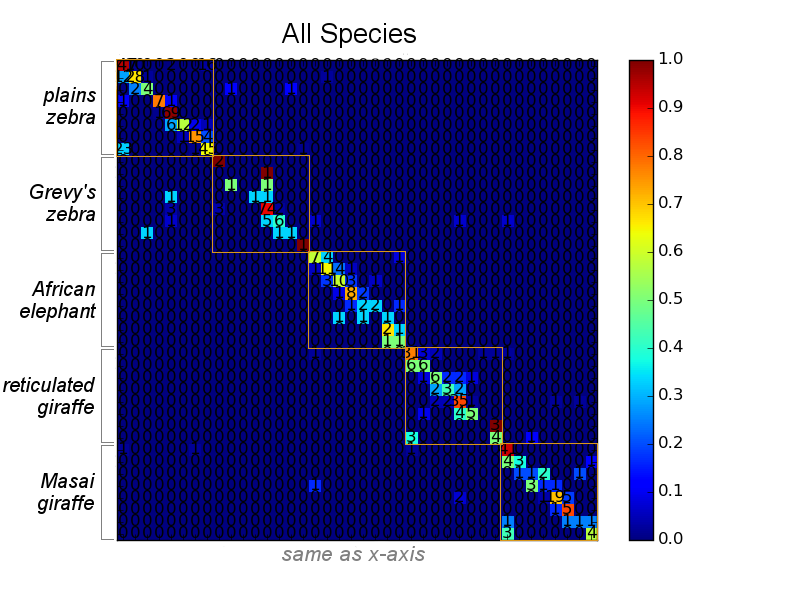
\includegraphics[width=0.85\textwidth]{resources/confusion-viewpoint-all-cleaned.png} }}$ }}%
        \caption[Confusion Matrix for All Species and Viewpoints]{\textbf{Confusion Matrix for All Species and Viewpoints.}  Patches of 5 species (plains zebra (1), Grevy's zebra (2), African elephant (3), reticulated giraffe (4), and Masai Giraffe (5)) and the 8 viewpoints for each species were used to train a 40-class DCNN.  The viewpoint order is the same as in Figure \ref{fig:confusion} (left).  Overall, most of the error is well contained within each species (and sub-species).}
        \label{fig:viewpoint-all}
\end{figure}

The classification of the quality scores, shown in Figure \ref{fig:features} (right), was a much noisier metric for the network to learn.  The network had difficulty because the subjective definition of quality caused much more confusion in the ground-truth.  However, one worthwhile result would be to learn a binary classification between annotations that were \textit{ok} or better against annotations that were worse than \textit{ok}.  The network was again given the same 8,860 quality-annotated images of plains zebra and was trained to distinguish between the 5 qualities: \textit{junk} (536), \textit{poor} (2270), \textit{ok} (3457), \textit{good} (1896), and \textit{excellent} (499).  In Figure \ref{fig:confusion} (right), the network had a much harder time differentiating between classes, but analyzing the error rate (white boxes) between classifying an annotation as \textit{ok} or better or otherwise the network achieves an overall accuracy of 78.39\%.  Looking closer, 4 out of 5 of the error cases (inside the white boxes) for the quality DCNN are isolated at the boundary between \textit{poor} and \textit{ok}.  Given the fuzziness of the manual annotations, we considered this accuracy to be sufficient for automatically providing quality scores to new images added to the system.

\section{GPS Verification}

\begin{figure}[!htb]%
    \centering
    \subfloat {{ $\vcenter{\hbox{ 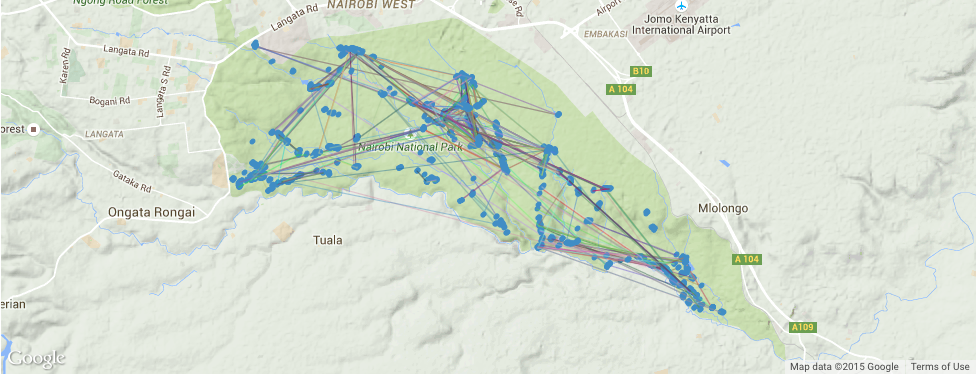
\includegraphics[width=0.90\textwidth]{resources/tracks.png} }}$ }}%
        \caption[Movement Tracks for Zebras in the Nairobi National Park]{\textbf{Movement Tracks for Zebras in the Nairobi National Park.}  The movement tracks from identified zebras in the Nairobi National Park shows the areas of concentration and the estimated tracks.  The colored dots indicate a sighting for a particular individual and the (identically colored) lines represent the connection between that individual's chronological sightings.  The time between sightings, and therefore the animal's speed, is not encoded in this representation.  The location of congregation tends to be in the middle of the park or near the southern, unfenced boundary of the park, which has better grazing conditions.  The approximated tracks indicate areas of estimated paths of travel.  With continued monitoring, a more complete picture of the population's movement can be used to help make conservation decisions to perserve the NNP's infratructure or to encourage or discourage movement thru specific areas.}
        \label{fig:tracks}
\end{figure}

To verify the GPS data collected during the GZGC, we analyzed the velocities between every sighting of every identified animal; speed values could be calculated between sightings of an individual by comparing a pair of GPS locations to find a distance value and dividing that by the time difference of the images.  The velocities of the animals were capped at a global maximum of  10 KPH and any animal exceeding that threshold was considered to have bad GPS or time data.  Each occurrence of an excessively speedy animal was flagged for further review.

For the purposes of reconciling the flagged animals, it was assumed that the string of GPS times and coordinate locations given by a particular dongle was reliably accurate and that the dongle was not otherwise malfunctioning.  Bad GPS data for an animal is then interpreted as a mis-synchronization of the time reported by the GPS dongle and the \textit{corrected} time for when the image was supposedly taken.   Therefore, flagged animals originate as an error that occurred during the image retrieval and image time synchronization process (detailed in Chapter \ref{sec:retrieval}).  The error during time synchronization propagates as a GPS error by the incorrect selection of an inappropriate corresponding GPS location reported by the dongle.  The time mis-synchronization could also be caused by an incorrect identification match.  Adequately performing name merges and splits, as explained in Chapter \ref{sec:identification}, will largely solve this issue before it becomes a problem during GPS verification.  However, name merge and split issues are unlikely to be completely resolved because they are difficult to detect.  Therefore, the GPS verification is a secondary detector for naming problems.  

To fix this synchronization, the time offset used for that citizen scientist, and all of their contributed images, must be altered to resolve the anomaly.  The time offset was incremented or decremented in time until the speed for that flagged occurrence was resolved, meaning it no longer violated the global speed limit.  However, the particular resolution (fixed time offset) for a specific flagged sighting was also applied to all images contributed by the same citizen scientist.  In practice, a specific resolution often fixed many of the flagged sightings for a particular contributor.  Unfortunately, the opposite case was also observed: where a time correction for a particular sighting caused a different sighting by the same participant to become unsynchronized, and subsequently flagged, due to now violating the speed threshold.  This phenomenon was the result of over- or under-shooting when correcting the time offset using only a single sighting and having a crude estimate for an animal's movement speed.  To fine-tune the offset, the procedure was repeated incrementally until all flagged animals were resolved for that individual citizen scientist.   In practice, only a few corrective iterations were required and no correction loops were observed.  A correction loop happens when a flagged sighting \textit{A} is corrected and results in a previously valid sighting \textit{B} to become flagged.  After correcting the newly flagged sighting \textit{B}, sighting \textit{A} becomes flagged again, causing a correction loop.  A correction loop would indicate that the global maximum speed threshold was either too low or a GPS dongle was malfunctioning.  This could violate the assumption that the GPS dongles all reported accurate information.

For the \textit{The Great Zebra \& Giraffe Count}, 5 participants were found to have flagged sightings.  These were successfully resolved and their GPS coordinates corrected by incrementing or decrementing their time offsets until they no longer violated the speed limit.  While this procedure is somewhat imprecise, we considered this to be an adequate estimation for the approximate location of the animals because the animals would most likely have stayed in the local vicinity for a short period of time.  For animals that were on the move, hopefully other sightings of that animal would cause future sightings to be flagged as obeying the speed limit.  This procedure was ultimately reliable because multiple photographers in a single car were able to corroborate sightings of an individual animal and serve, in essence, as each other's time alibi.  A car without multiple photographers must rely on having a re-sighting of an individual animal by another photographer in another car, which may be a difficult constraint to satisfy.  Luckily, the images contributed to the GZGC were all provided with other sightings for when ambiguities arose.

In summary, the labeling networks were very effective at automatically assigning species and viewpoint labels.  The quality labeling network was not as accurate at modeling the very subjective metric.  However, for the purposes of the GZGC and the IBEIS identification system, the quality was sufficient for assigning a suitable threshold for \textit{ok} or better.  The networks led to the identification of incorrectly assigned species and viewpoints in the recognition database, which improved overall accuracy and identification speed.  For future data collection events, the species and viewpoint DCNN can be used to simplify the submission client by automatically suggesting the dominant species in the image or be used to remove that requirement by doing the detection and inference server side.  The DCNN architectures used for species and viewpoint classification also give hope that the classifier could be used to power a DCNN-based detector, which would be naturally multi-class and very efficient at performing inference across an entire input image.  This proposed DCNN-based detector will be the focus of future research.
